% Options for packages loaded elsewhere
\PassOptionsToPackage{unicode}{hyperref}
\PassOptionsToPackage{hyphens}{url}
%
\documentclass[
]{article}
\usepackage{amsmath,amssymb}
\usepackage{iftex}
\ifPDFTeX
  \usepackage[T1]{fontenc}
  \usepackage[utf8]{inputenc}
  \usepackage{textcomp} % provide euro and other symbols
\else % if luatex or xetex
  \usepackage{unicode-math} % this also loads fontspec
  \defaultfontfeatures{Scale=MatchLowercase}
  \defaultfontfeatures[\rmfamily]{Ligatures=TeX,Scale=1}
\fi
\usepackage{lmodern}
\ifPDFTeX\else
  % xetex/luatex font selection
\fi
% Use upquote if available, for straight quotes in verbatim environments
\IfFileExists{upquote.sty}{\usepackage{upquote}}{}
\IfFileExists{microtype.sty}{% use microtype if available
  \usepackage[]{microtype}
  \UseMicrotypeSet[protrusion]{basicmath} % disable protrusion for tt fonts
}{}
\makeatletter
\@ifundefined{KOMAClassName}{% if non-KOMA class
  \IfFileExists{parskip.sty}{%
    \usepackage{parskip}
  }{% else
    \setlength{\parindent}{0pt}
    \setlength{\parskip}{6pt plus 2pt minus 1pt}}
}{% if KOMA class
  \KOMAoptions{parskip=half}}
\makeatother
\usepackage{xcolor}
\usepackage{longtable,booktabs,array}
\usepackage{calc} % for calculating minipage widths
% Correct order of tables after \paragraph or \subparagraph
\usepackage{etoolbox}
\makeatletter
\patchcmd\longtable{\par}{\if@noskipsec\mbox{}\fi\par}{}{}
\makeatother
% Allow footnotes in longtable head/foot
\IfFileExists{footnotehyper.sty}{\usepackage{footnotehyper}}{\usepackage{footnote}}
\makesavenoteenv{longtable}
\usepackage{graphicx}
\makeatletter
\def\maxwidth{\ifdim\Gin@nat@width>\linewidth\linewidth\else\Gin@nat@width\fi}
\def\maxheight{\ifdim\Gin@nat@height>\textheight\textheight\else\Gin@nat@height\fi}
\makeatother
% Scale images if necessary, so that they will not overflow the page
% margins by default, and it is still possible to overwrite the defaults
% using explicit options in \includegraphics[width, height, ...]{}
\setkeys{Gin}{width=\maxwidth,height=\maxheight,keepaspectratio}
% Set default figure placement to htbp
\makeatletter
\def\fps@figure{htbp}
\makeatother
\setlength{\emergencystretch}{3em} % prevent overfull lines
\providecommand{\tightlist}{%
  \setlength{\itemsep}{0pt}\setlength{\parskip}{0pt}}
\setcounter{secnumdepth}{-\maxdimen} % remove section numbering
\ifLuaTeX
  \usepackage{selnolig}  % disable illegal ligatures
\fi
\IfFileExists{bookmark.sty}{\usepackage{bookmark}}{\usepackage{hyperref}}
\IfFileExists{xurl.sty}{\usepackage{xurl}}{} % add URL line breaks if available
\urlstyle{same}
\hypersetup{
  hidelinks,
  pdfcreator={LaTeX via pandoc}}

\author{}
\date{}

\begin{document}

\section{Task 1}\label{task-1}

\section{a)}\label{a}

\begin{enumerate}
\def\labelenumi{\arabic{enumi}.}
\item
  Location of the new station
\end{enumerate}

The new SHEPSHED station is located in eastern suburbs of the town, an
area with sparse residential development, which circumvents the high
demolition costs typically associated with urban station constructions.
Crucially, its position ensures that the vast majority of the town is
accessible within a 2000-metre radius, making it an optimal site for the
station.

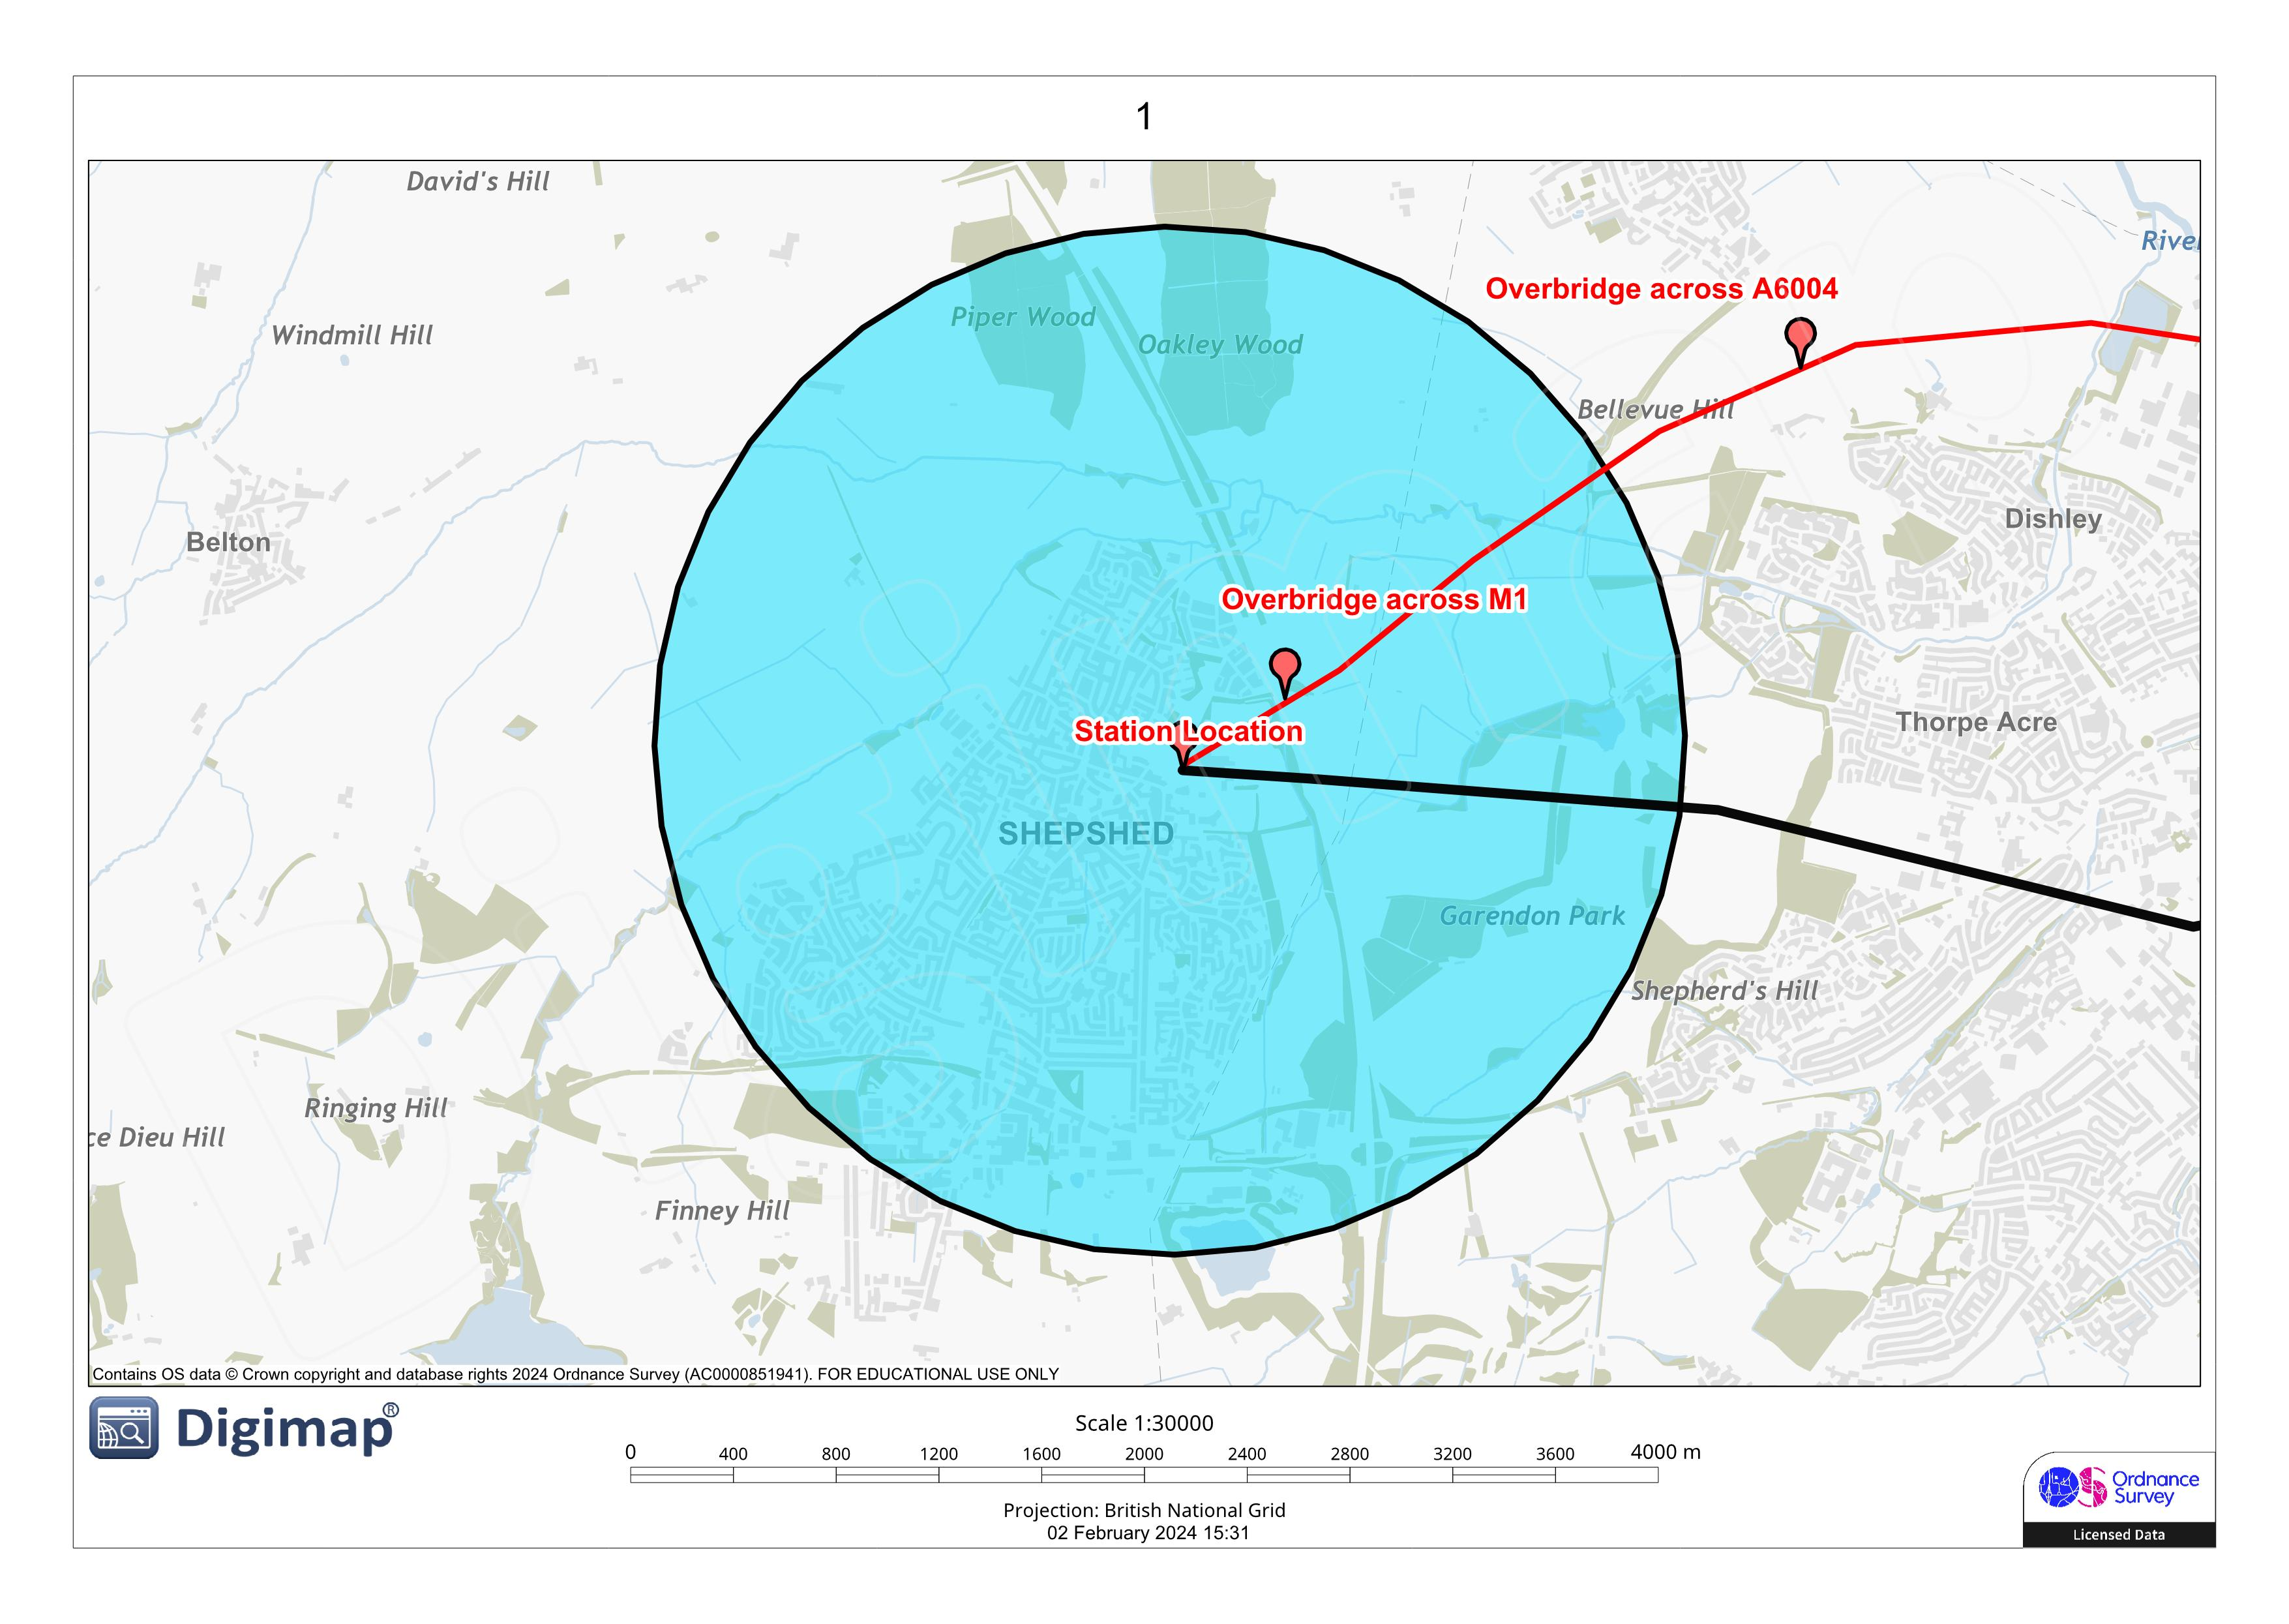
\includegraphics{C:/Users/18117/Pictures/digimap_roam.jpg}

\begin{enumerate}
\def\labelenumi{\arabic{enumi}.}
\item
  Route direction
\end{enumerate}

The proposed route outlined in red in Fig X, bypassed Loughborough to
the north. The detour, while lengthening the journey and navigating
challenging elevations in the northwest, significantly increases
construction costs with respect to excavation and filling works.
However, this route minimizes disruptions to the urban road network,
meeting key stakeholder expectations. Importantly, it enhances
operational efficiency by eliminating the need for speed reductions at
Loughborough Central Station, a critical advantage for maintaining
optimal transit times. This alignment represents a deliberate trade-off,
prioritizing operational and community benefits over the increased
direct costs and construction complexities.

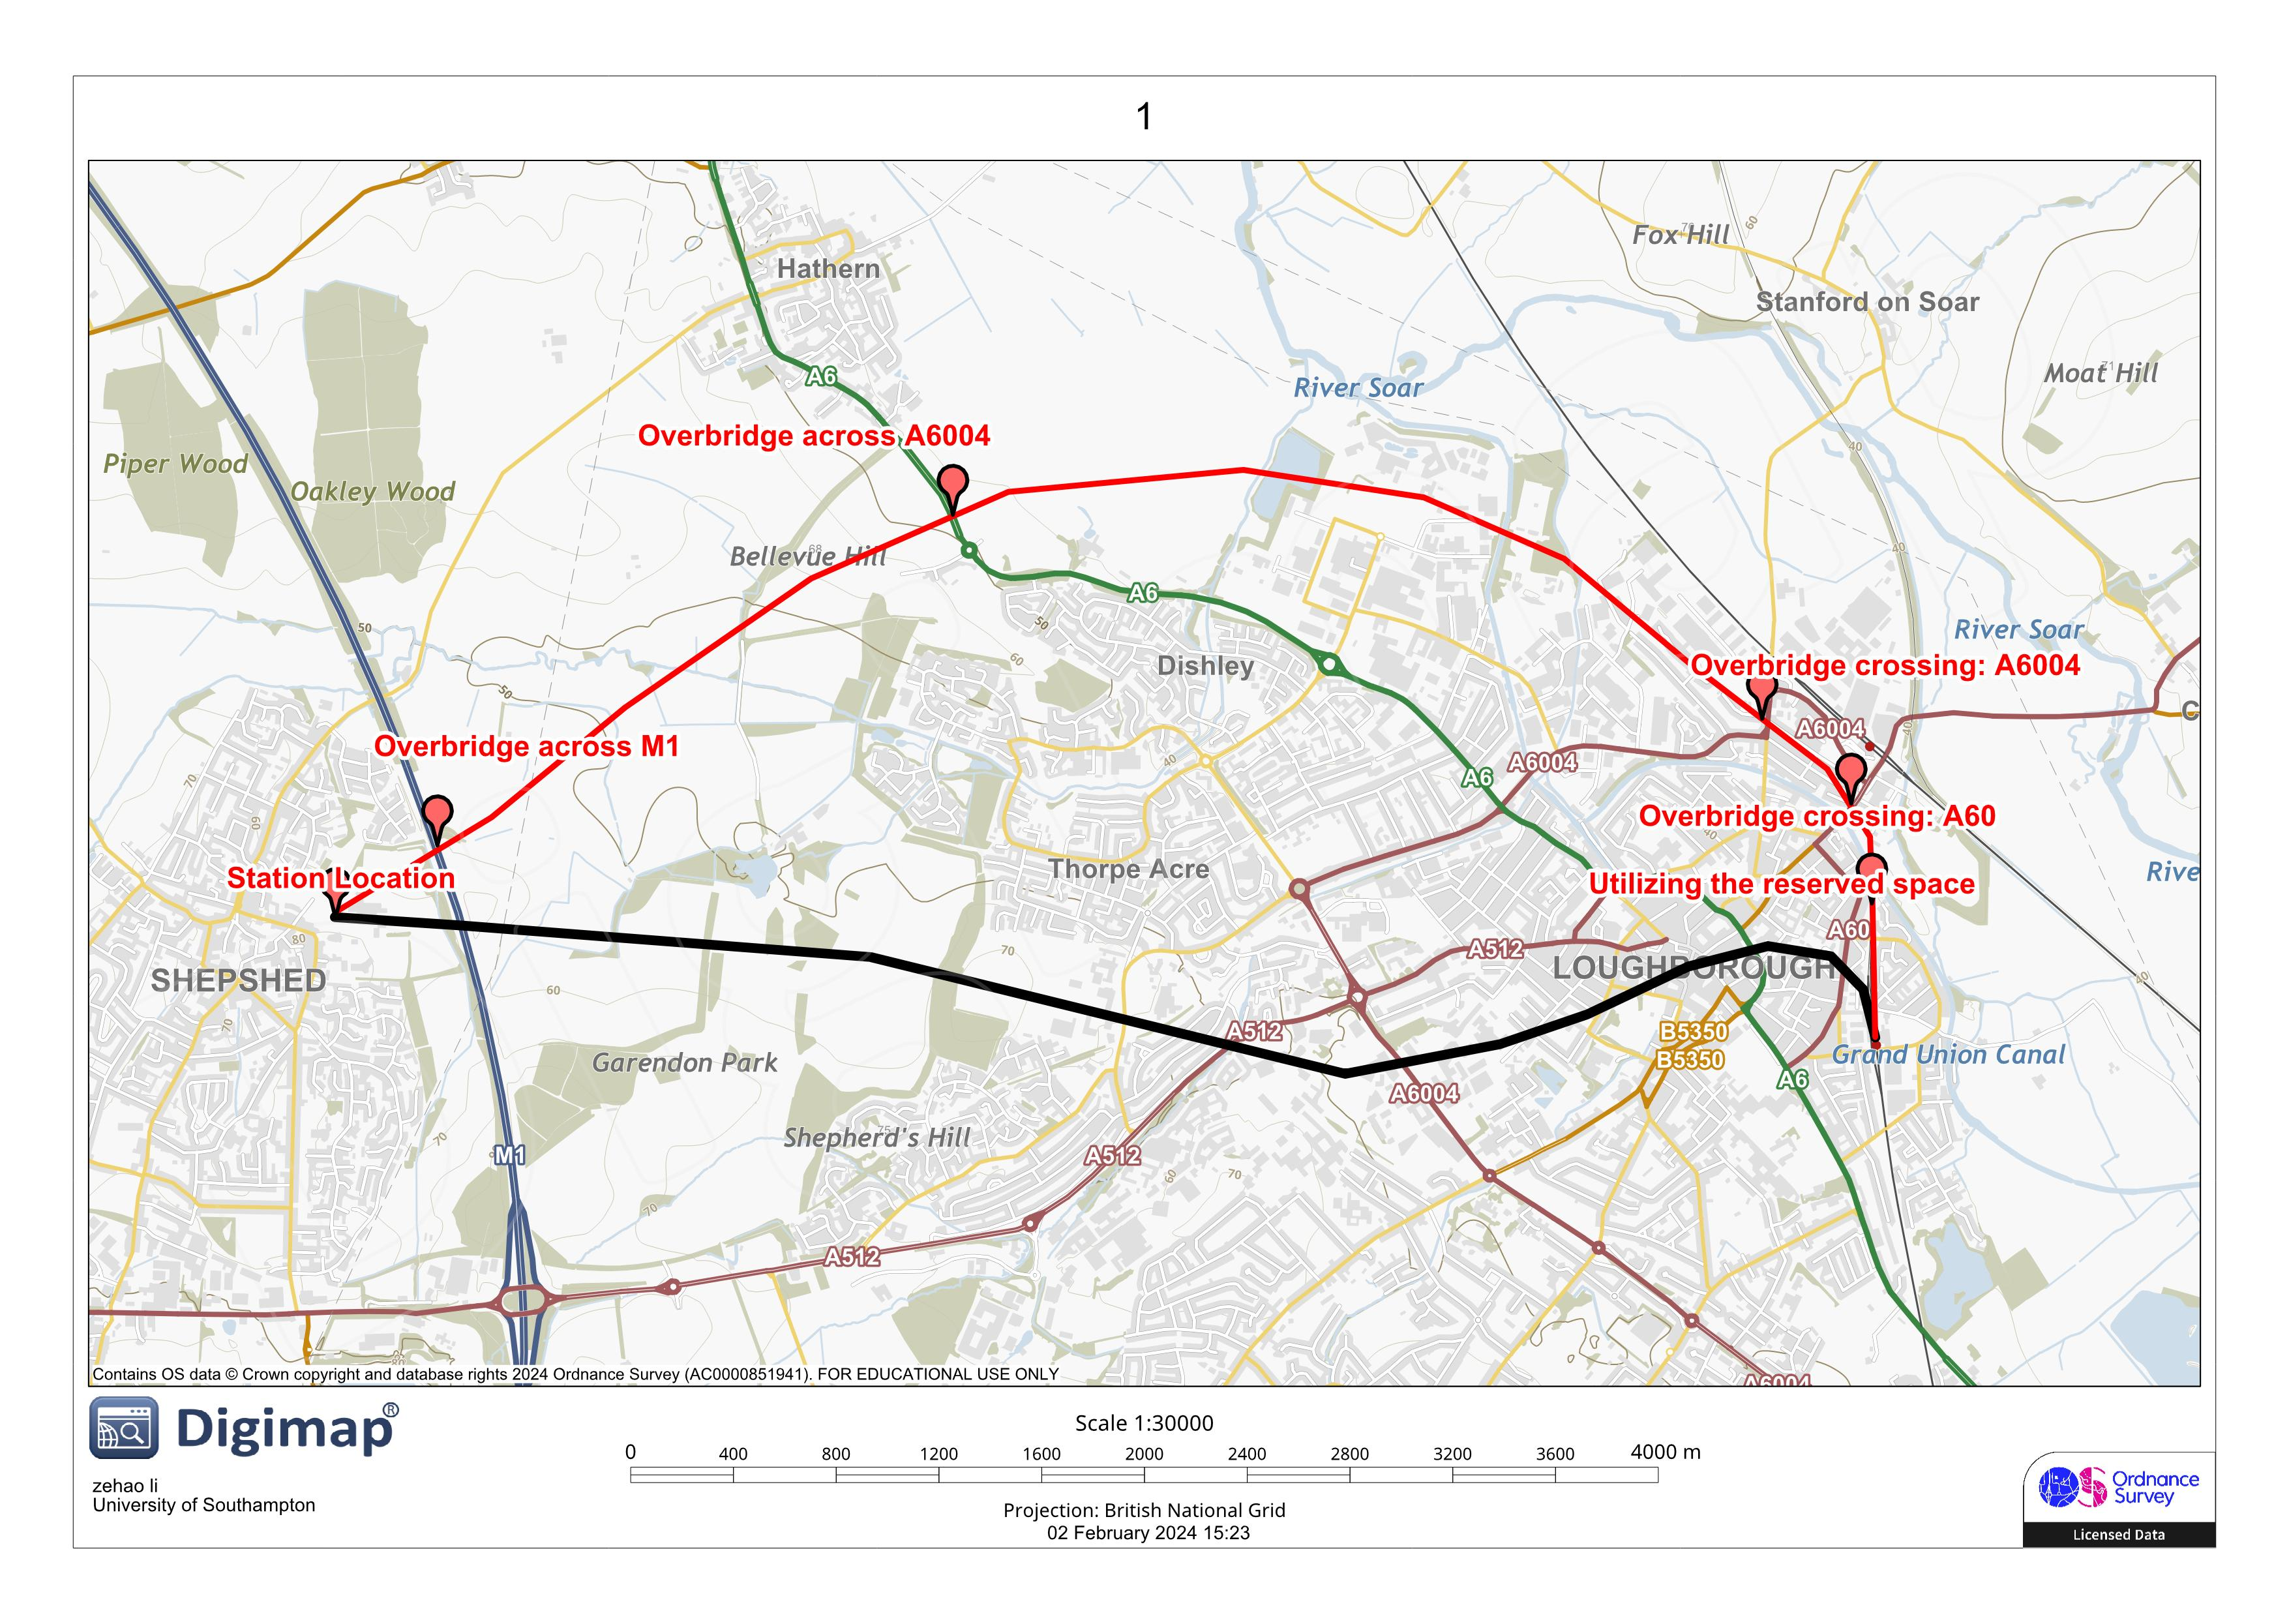
\includegraphics{C:/Users/18117/Pictures/digimap_roam-20240202-0323.jpg}

\begin{enumerate}
\def\labelenumi{\arabic{enumi}.}
\item
  key control points
\end{enumerate}

The design incorporates two types of control points to seamlessly
integrate with existing infrastructure:

\begin{enumerate}
\def\labelenumi{\arabic{enumi}.}
\item
  \textbf{At Road Intersections}: To maintain traffic flow on major
  roads, the design replaces level crossings at intersections with
  bridges over the M1, A6004(west and east sides), and A60. This choice,
  although increasing construction costs, is justified by the
  bridges\textquotesingle{} minimal disruption to existing traffic
  patterns. By prioritizing bridges, the design significantly mitigates
  interference with the traffic infrastructure, demonstrating a balanced
  approach to cost and community impact.
\end{enumerate}

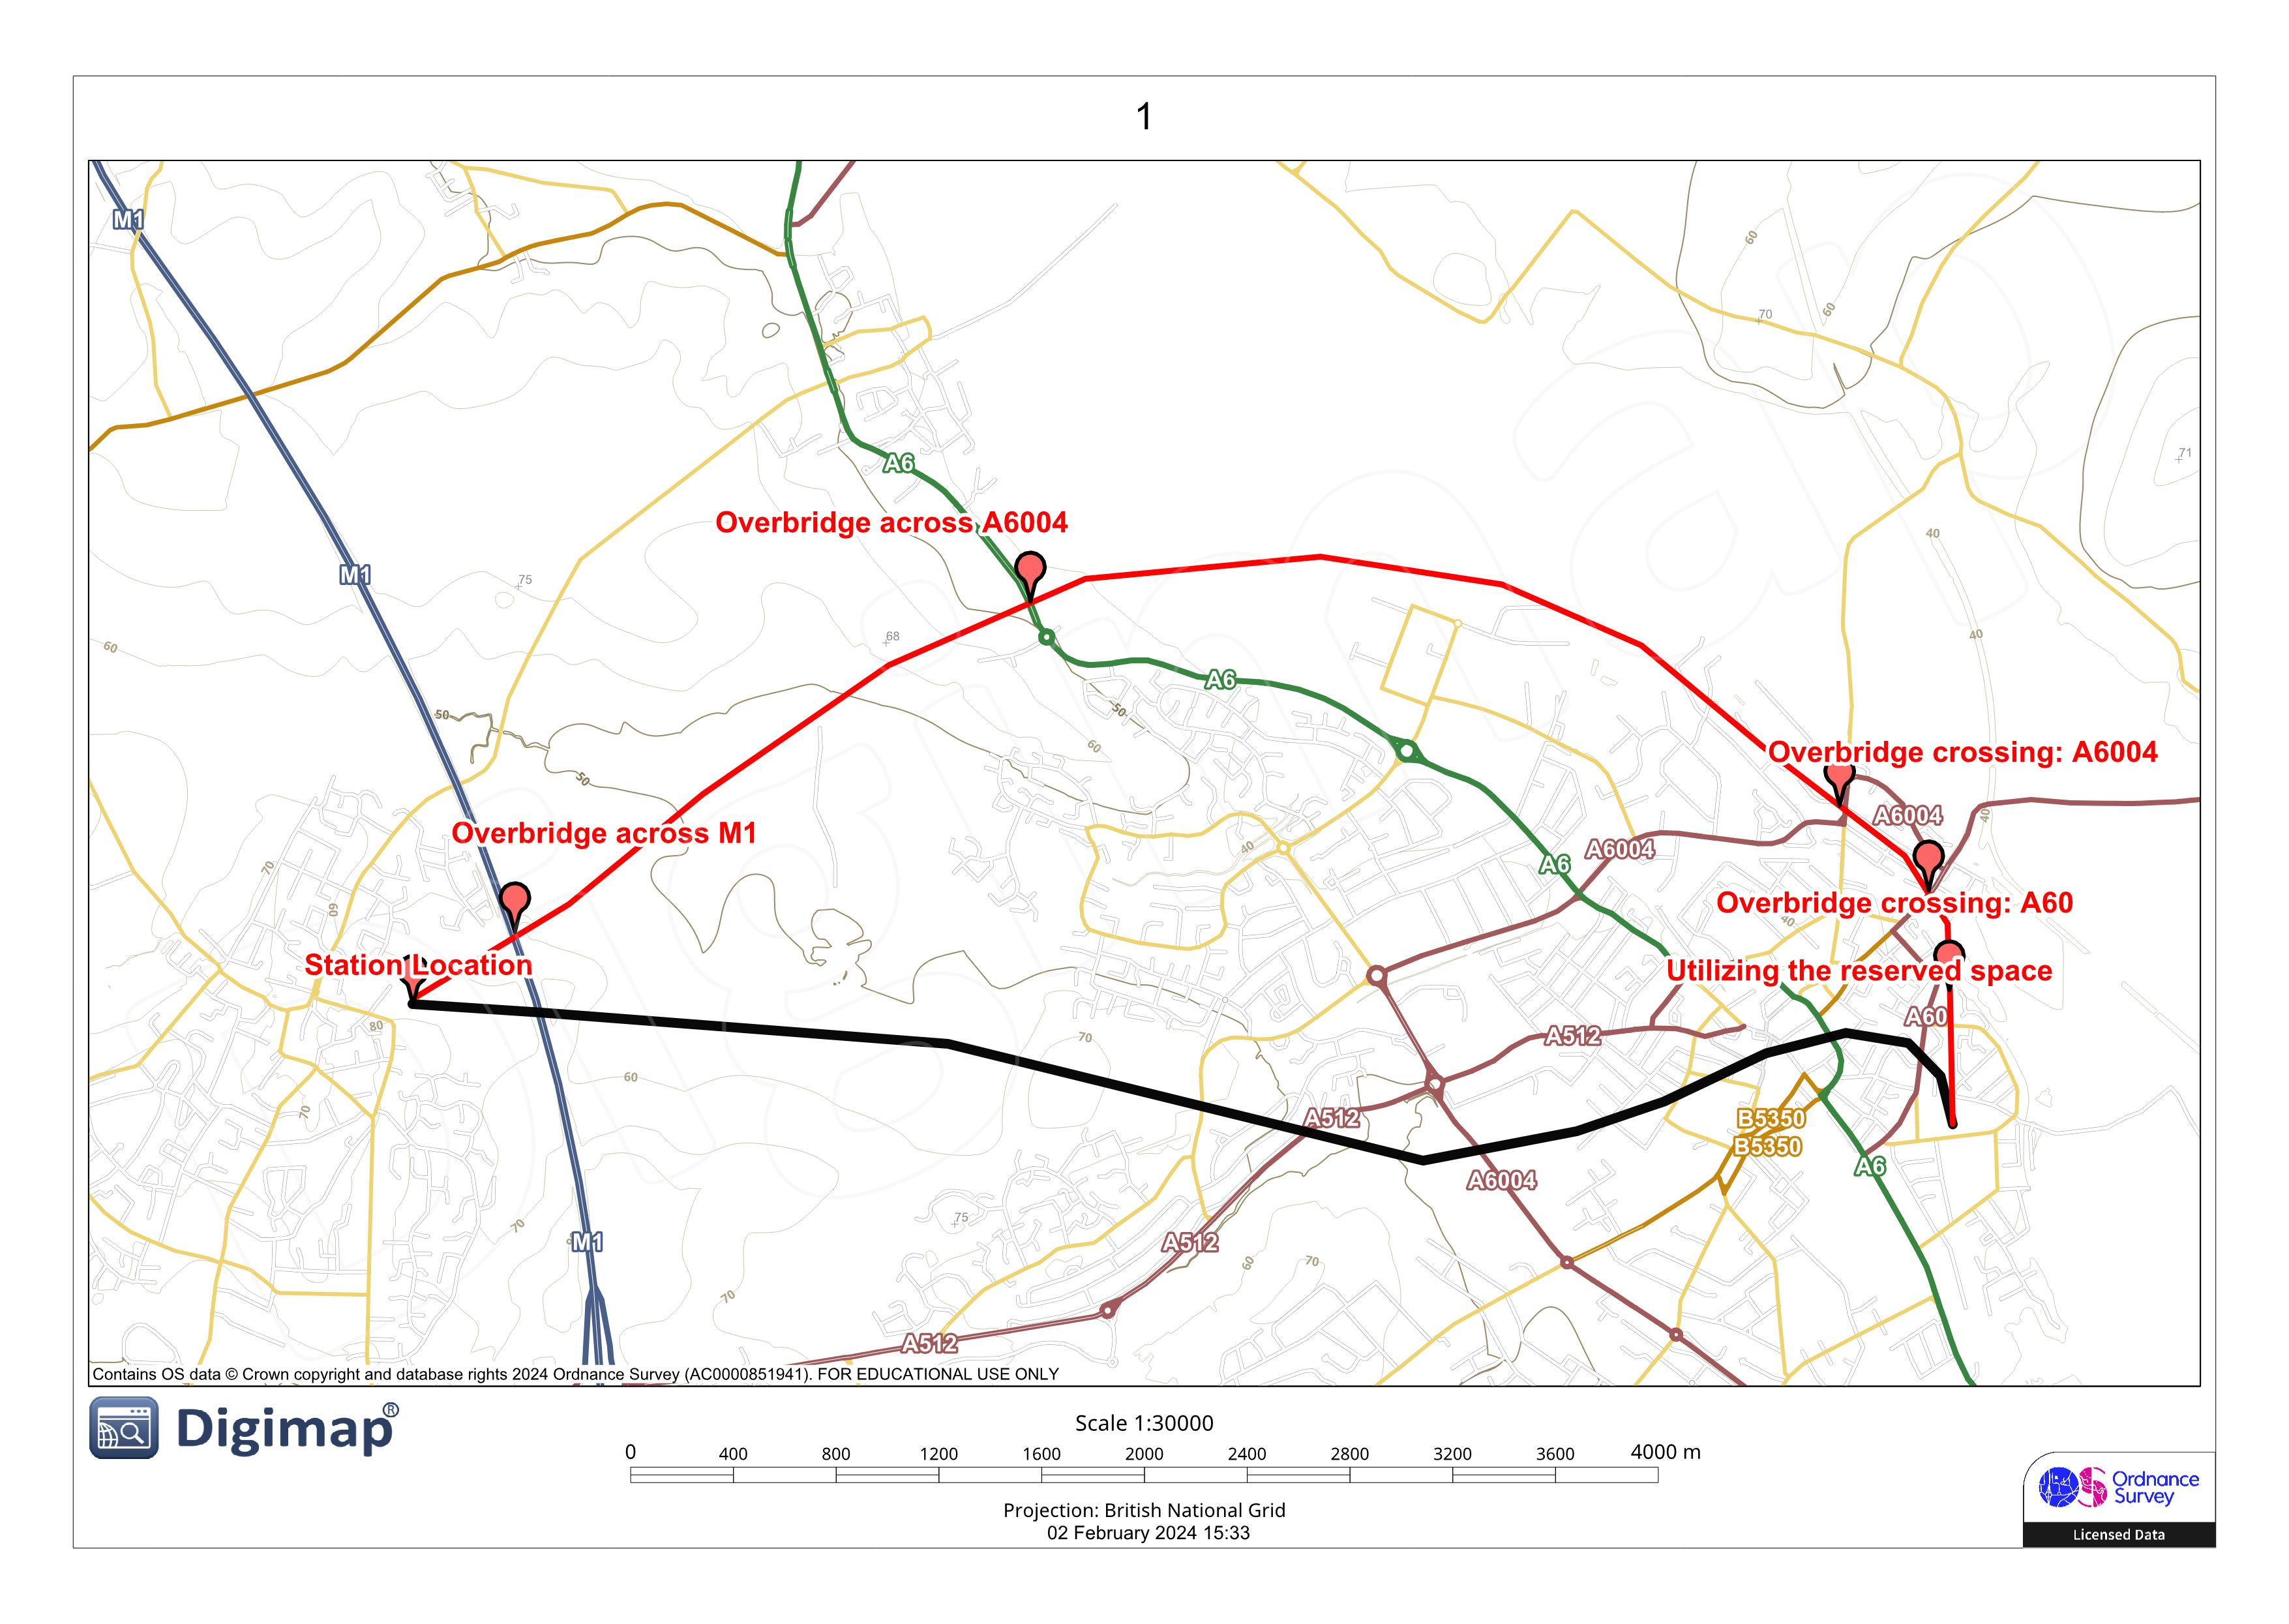
\includegraphics{C:/Users/18117/Pictures/digimap_roam (1).jpg}

\begin{enumerate}
\def\labelenumi{\arabic{enumi}.}
\item
  \textbf{In Rail Connections}: Strategically, the design leverages the
  reserved rail line on the north side of Loughborough Central Station,
  which is possibly prepared for future connection with the northern
  Loughborough Station. This integration significantly reduces costs by
  utilizing the reserved space and improves operational efficiency
  through a smoother line shape.
\end{enumerate}

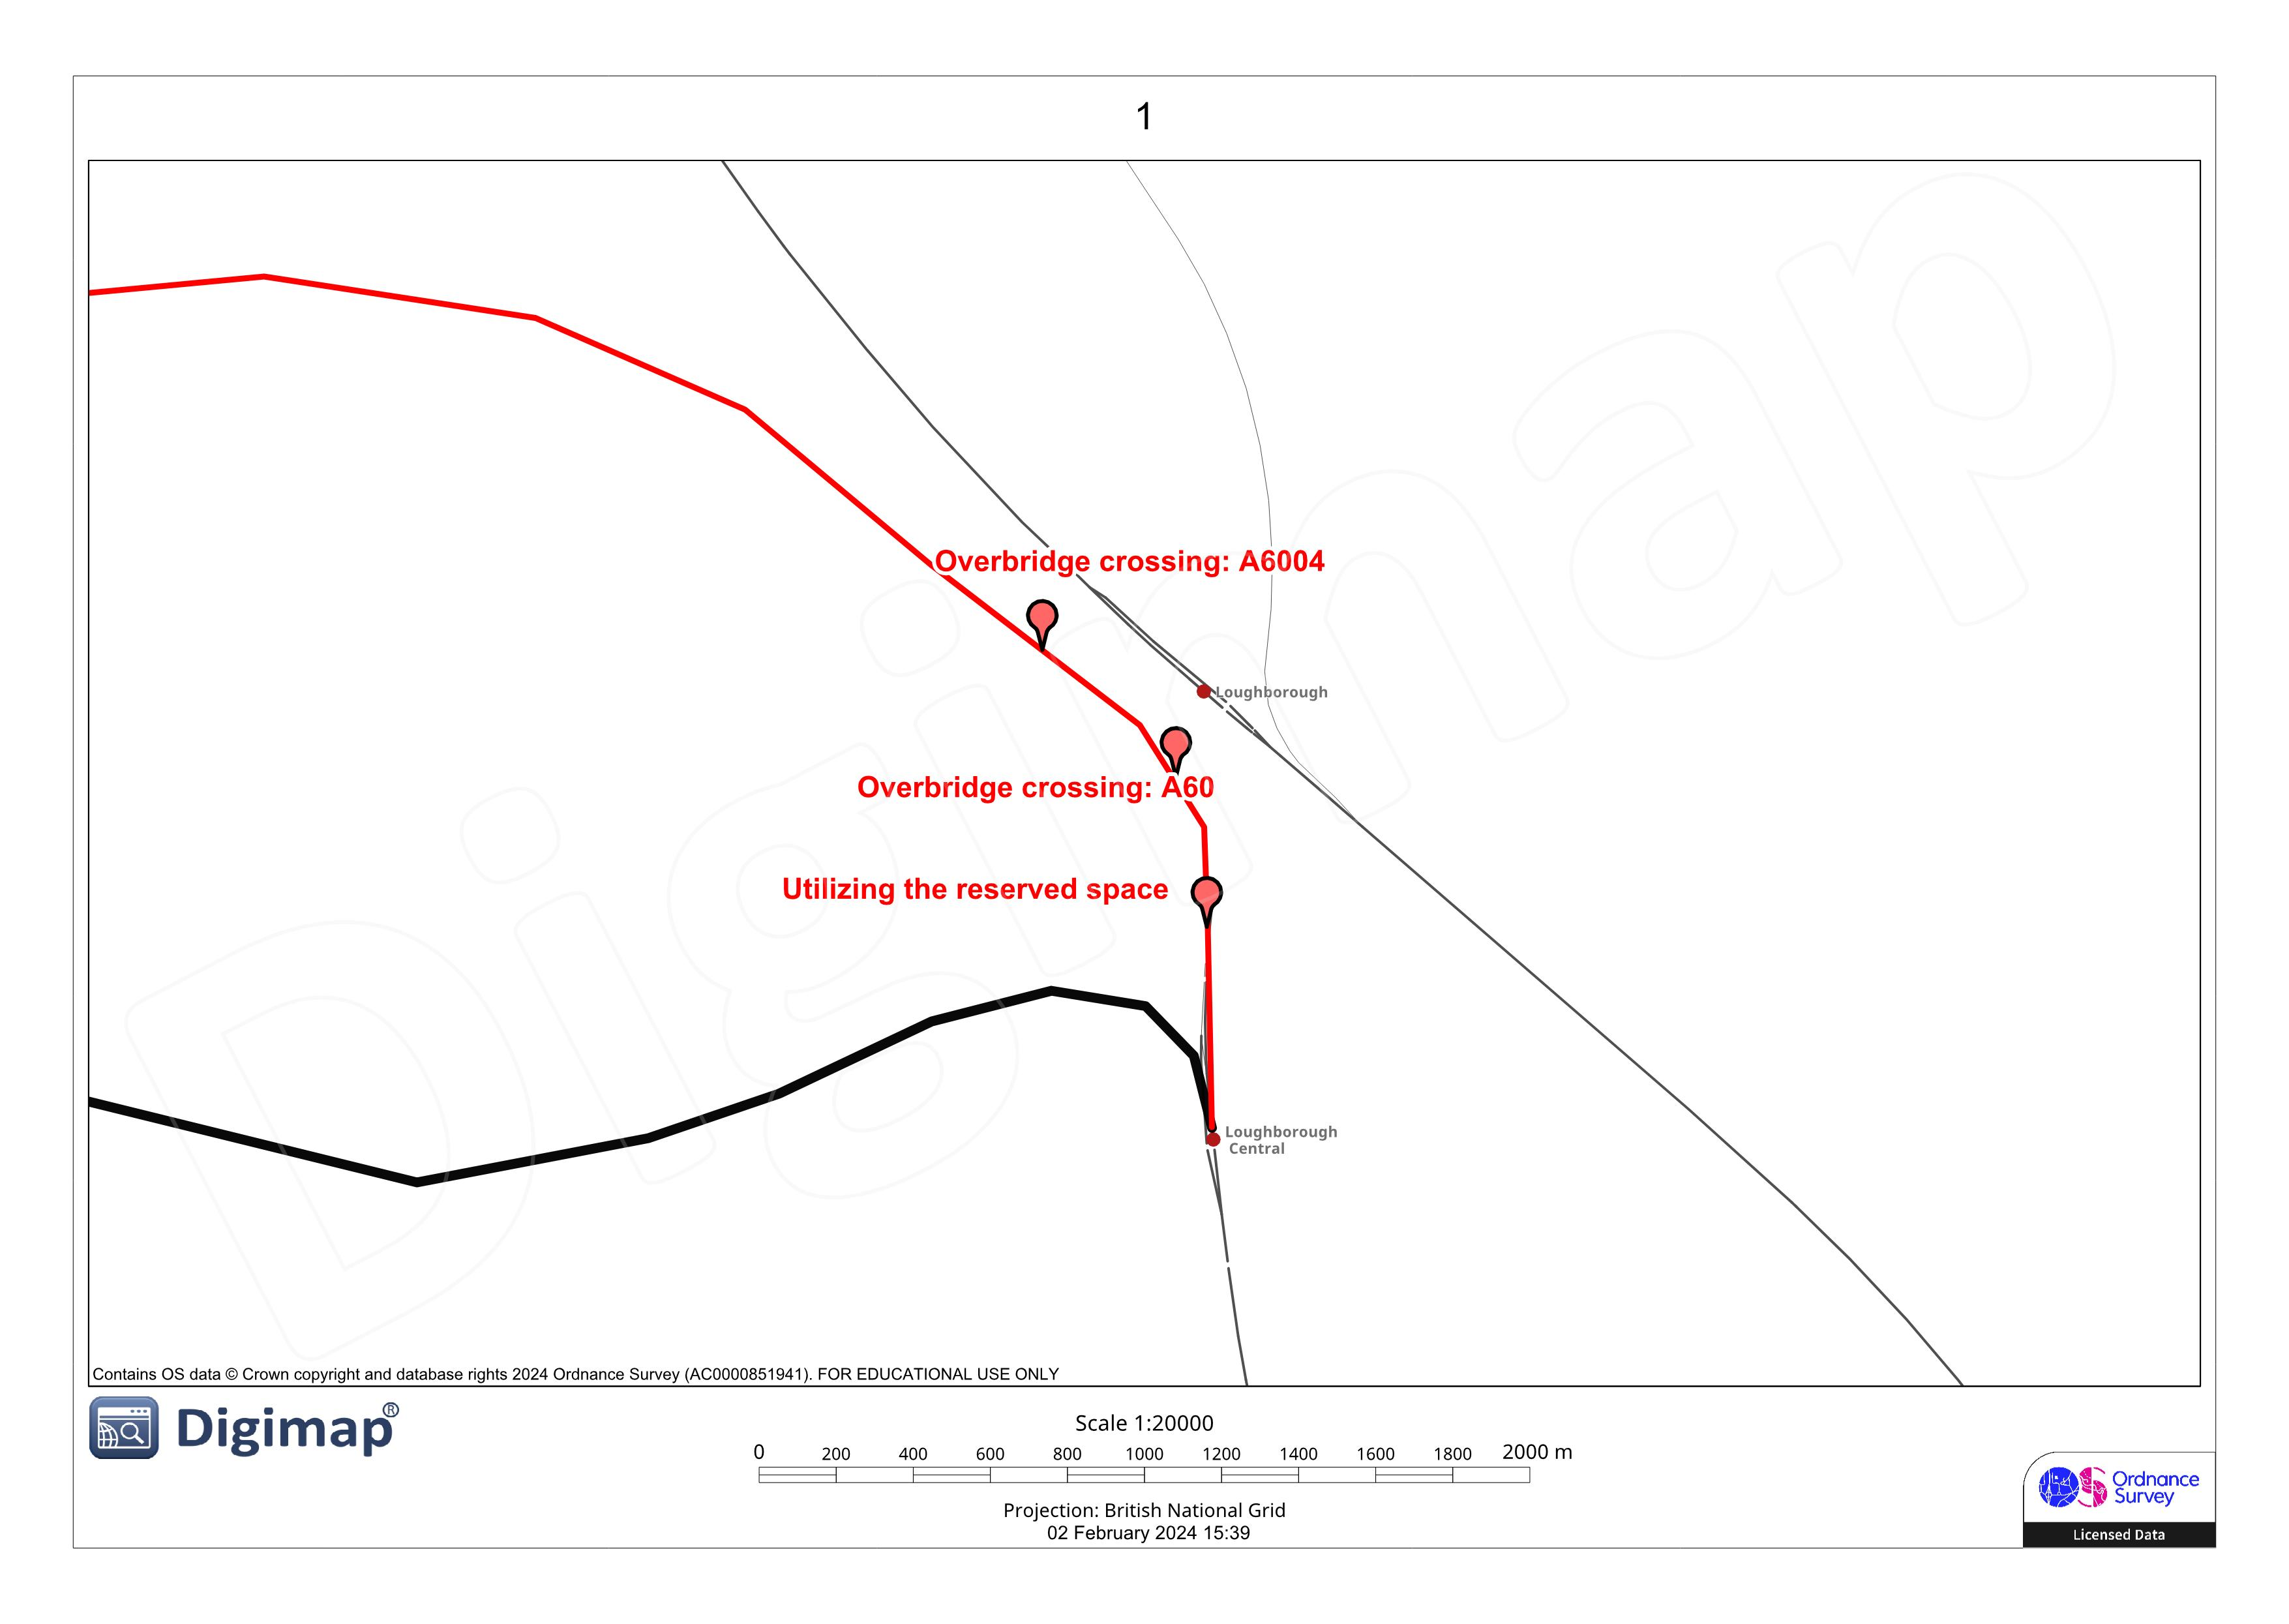
\includegraphics{C:/Users/18117/Pictures/digimap_roam (5).jpg}

\section{b)}\label{b}

\includegraphics{C:/Users/18117/Pictures/CUb1ljgfhsfHf7Hsvs\%2BoUk1s9PsQNAODsaAVxAWk\%3D}

Based on the obtained contour data, a gradient profile shown in Fig X is
recommended, adhering to a maximum ratio of 1:50(for sections up to
3km). The profile reveals significant gradient changes, necessitating
extensive earthwork. Such work increases costs and adversely affects the
environment.

To mitigate these impacts, it is suggested to construct a tunnel
approximately 800 metres long at the most challenging mountain segment,
located between 2000 and 2500 meters along the route.

\section{c)}\label{c}

By using the online tool Station Demand Forecasting Tool, it is
predicted that the number of passengers using the new station in its
year of opening year is 905215. The follow figures show the station
location and the road access point.

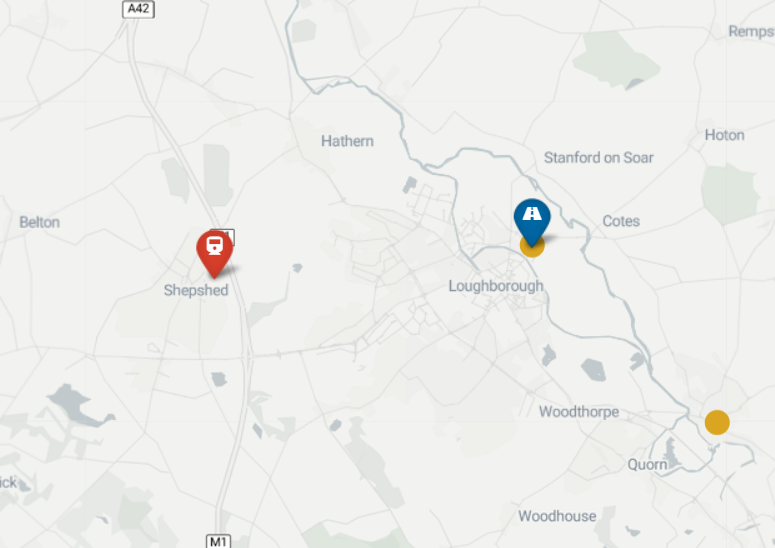
\includegraphics{C:/Users/18117/Pictures/image-20240203120054780.png}

The input values are shown in Table 1 and it should be noted that the
Frequency is calculated using the following formula:

\begin{flalign}
\text{Frequency} &= 2 \times \left(\frac{\text{total\_run\_time\_minutes}}{\text{interval\_minutes}} + 1\right) && \\
                 &= 2 \times \left(\frac{18 \times 60}{40} + 1\right) && \\
                 &= 56 &&
\end{flalign}

\begin{longtable}[]{@{}ll@{}}
\toprule\noalign{}
id & 3812 \\
\midrule\noalign{}
\endhead
\bottomrule\noalign{}
\endlastfoot
name & SHEPSHED \\
region & East Midlands \\
station\_easting & 448381 \\
station\_northing & 319786 \\
access\_easting & 454346 \\
access\_northing & 319361 \\
frequency & 56 \\
frequency\_group & NA \\
parking\_spaces & 100 \\
ticket\_machine & TRUE \\
bus\_interchange & TRUE \\
cctv & TRUE \\
terminal\_station & TRUE \\
travelcard\_boundary & FALSE \\
category & E \\
\end{longtable}

\section{d)}\label{d}

For commuters:

\begin{align*}
\text{Commuter Ratio} & = \left(\frac{8.7}{8.25}\right)^{-0.6} \times \left(\frac{26+23}{26+27}\right)^{-0.6} \\
\text{Commuters in base year} & = 0.40 \times 905215 \\
\text{Commuters in 2035} & = \text{Commuters in base year} \times \text{Commuter Ratio}
\end{align*}

For business:

\begin{align*}
\text{Business Ratio} & = \left(\frac{8.7}{8.25}\right)^{-0.7} \times \left(\frac{26+23}{26+27}\right)^{-0.6} \\
\text{Business Travelers in base year} & = 0.15 \times 905215 \\
\text{Business Travelers in 2035} & = \text{Business Travelers in base year} \times \text{Business Ratio}
\end{align*}

For leisure:

\begin{align*}
\text{Leisure Ratio} & = \left(\frac{8.7}{8.25}\right)^{-1.3} \times \left(\frac{26+23}{26+27}\right)^{-0.6} \\
\text{Leisure Travelers in base year} & = 0.45 \times 905215 \\
\text{Leisure Travelers in 2035} & = \text{Leisure Travelers in base year} \times \text{Leisure Ratio}
\end{align*}

Therefore, the number of travelers in 2035 is 903271.

\section{Task 2}\label{task-2}

\subsection{1)}\label{1}

Based on Task 1, the frequency of trains passing through this route has
been calculated. If we consider only one direction (for example, from
Shepshed to Loughborough), there are 28 train services per day.
Therefore, we can calculate the annual number of vehicle passes from
Shepshed to Loughborough as follows:

\[the\ annual\ number\ of\ vehicles\ passes=3\times365\times28=30660\]

According to the results found on the official website, there are 41
train services from Southampton Airport Parkway to London Waterloo per
day, resulting in an annual number of vehicle passes of 44,895.
Comparing this with the new route design, we can observe two main
differences in the train service from Southampton to London. First, the
frequency of trains increases during peak hours in the morning and
evening. Second, at certain times within these peak periods, the service
operates two trains simultaneously---one fast and one slow. This design
is flexible, tailoring the frequency and intervals of departures to meet
varying travel demands at different times. It\textquotesingle s an
approach worth learning from and applying
elsewhere.\includegraphics{C:/Users/18117/Pictures/image-20240212101026605.png}

\begin{quote}
\href{https://ojp.nationalrail.co.uk/service/pockettimetable/search}{Your
Pocket Timetables - National Rail Enquiries}
\end{quote}

\subsubsection{2)}\label{2uxff09}

In total, there are two types of soil failure the methodology is
designed to prevent, Subgrade Progressive Sheer Failure and Excessive
Subgrade Plastic Deformation, which can be represented by the following
two figures.

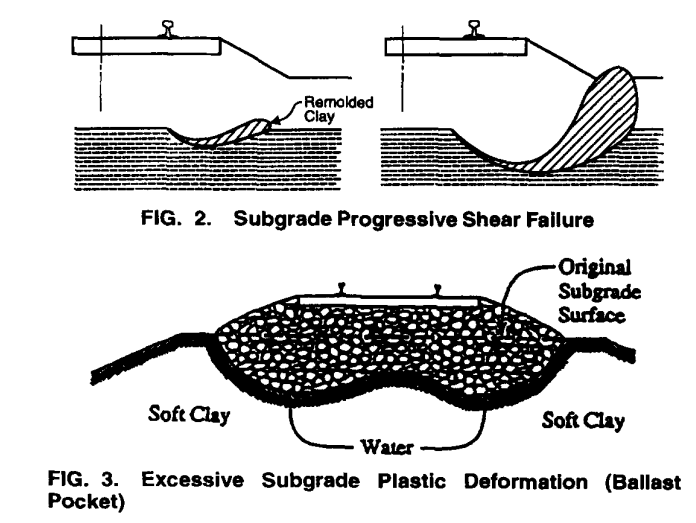
\includegraphics{C:/Users/18117/Pictures/image-20240212155516399.png}

Since we\textquotesingle re using the fat clay(CH), the parameters are
as follows: a=1.2, b=0.18, and m=2.4. The formula given is:

\[\epsilon=1.2(\frac{\sigma_d}{\sigma_s})^{2.4}*N^{0.18}\]

\includegraphics{C:/Users/18117/Pictures/vJ3U\%3D}

\[\frac{\sigma_d}{\sigma_s} \approx 0.586, 0.520, 0.461, 0.437\\
\because \sigma_s=65\ kPa\\
\therefore \sigma_d\approx38.09,33.8,29.965,28.405 kPa\\
DAF=1+0.052\times150/3.6/1=3.1667\\
P_d=DAF\times100=316.67kN\\
\therefore I=0.645\times\sigma_d/P_d\]

\includegraphics{C:/Users/18117/Pictures/image-20240203103232902.png}

\includegraphics{C:/Users/18117/Pictures/1.png}

The final thickness is derived from the figure and is shown in the
table:

\begin{longtable}[]{@{}lllllll@{}}
\toprule\noalign{}
vehicle passes & & & I & H/L & H & Time(year) \\
\midrule\noalign{}
\endhead
\bottomrule\noalign{}
\endlastfoot
200000 & 0.586 & 38.09 & 0.201928625 & 2.65 & 0.4028 & 6.523157208 \\
1000000 & 0.52 & 33.8 & 0.17918581 & 3.19 & 0.48488 & 32.61578604 \\
5000000 & 0.461 & 29.965 & 0.158855113 & 4.03 & 0.61256 & 163.0789302 \\
10000000 & 0.437 & 28.405 & 0.150584998 & 4.56 & 0.69312 &
326.1578604 \\
\end{longtable}

Assuming that ballast is replaced once every 30 years, I would suggest
that a ballast thickness of 0.48m be used, a value that strikes a
balance between engineering cost and durability.

\subsection{3)}\label{3uxff09}

The majority of the bedrock geology along the entire route is
Mudstone(with subordinate dolomitic siltstone and fine-grained
sandstone). The surface layer consists of Till, a mixture made up of
clay and large rocks.

\includegraphics{C:/Users/18117/Pictures/image-20240212164427626.png}

\includegraphics{C:/Users/18117/Pictures/image-20240212164449508.png}

Due to the presence of clay at the surface, there\textquotesingle s a
higher likelihood of shear failure and excessive plastic deformation.
This can be described using the Li and Selig method(This means that the
shear strength Es is relatively small and can be taken as one of 14, 28,
55 or 110 MPa).

\subsection{4)}\label{4uxff09}

For granular subgrades, such as sands and gravels, or underlying rock,
their strength is significantly higher than that of clay, making them
less prone to progressive shear failure or excessive deformation due to
deviator stress. As a result, the methods discussed in the paper are not
suitable for these types of subgrades. When designing for these
materials, one should consider the thickness of the granular layer from
the perspective of other types of failures, such as slope stability
collapse or excessive consolidation settlement caused by the
material\textquotesingle s self-weight. For instance, by setting a
critical value for a specific stress or strain indicator based on the
critical conditions under which these problems occur, the designed
thickness should ensure that the operational values of these indicators
remain below the critical thresholds.

\section{Task 3}\label{task-3}

\subsection{a)}\label{a-2}

This new line is a short addition, about 7 kilometers (roughly 4.3
miles) in length, dedicated to passenger transport. Consequently,
we\textquotesingle ve chosen the C1 type passenger vehicle standard
gauge as outlined in "The V/S SIC Guide to British Gauging Practice."
The C1 gauge is designed specifically for standard-length passenger
vehicles, about 20 meters (approximately 65 feet) long, though versions
for shorter vehicles also exist. These vehicles typically feature
traditional metal spring suspension systems, with a standard bogie
center spacing of 14 meters. Details about the vehicle design and gauge
limits are illustrated in the accompanying diagram.

\begin{quote}
\url{http://www.rssb.co.uk/Library/groups-and-committees/2013-guide-vehicle-structure-sic-guide-to-british-gauging-t926.pdf}
\end{quote}

\includegraphics{C:/Users/18117/Pictures/image-20240216160646416.png}

For the tunnel constructed at the 2000-meter mark of the new line,
it\textquotesingle s crucial to maintain a minimum distance of 100mm
between the vehicle\textquotesingle s loading gauge and the tunnel,
which is the recommended clearance. This ensures that, even under the
most adverse conditions, there\textquotesingle s no risk of collision, a
vital consideration for passenger safety. Maintaining infrastructure is
equally critical to prevent deformation that could result in
insufficient clearance.

Note that building a vehicle that truly meets C1 and can actually
operate is going to be quite a challenge. This is mainly because air
suspension allows for much more movement of the vehicle body than
traditional steel springs do. Therefore, providing enough infrastructure
space to accommodate suspension movement at all positions would be very
costly. As a result, a dynamic measurement process was developed to
allow the introduction of vehicles with air suspension.

\section{b)}\label{b-2}

Based on the data retrieved from the Geoindex, along the predetermined
route, there are two types of bedrock present. The first half of the
route features mudstone, while the second half consists of both mudstone
and siltstone. For the purposes of this analysis, the bedrock condition
in the first half of the route is classified under the category of
Murcia Mudstone:

\[\phi=30\\

c=5\\

\gamma=20\]

For determining the elevation and slope, according to the route map,
it\textquotesingle s noted that at the 500-meter mark, there is a need
to cross the M1 motorway. This will require an embankment(silt, clay)
project. It can be assumed:

\[\beta = 15\ degrees,H = 6m\]

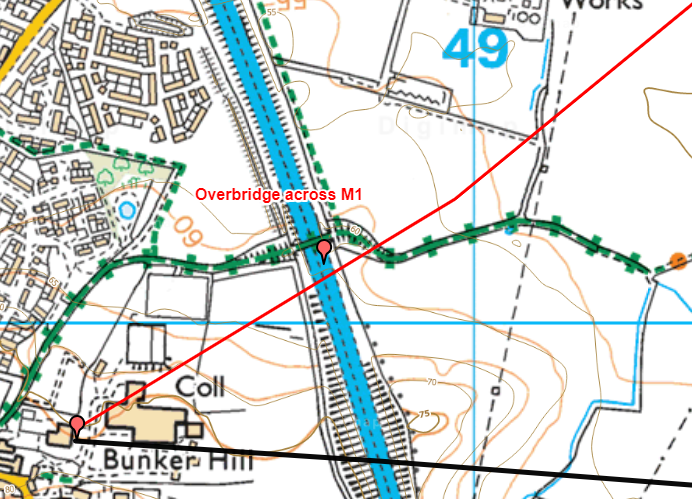
\includegraphics{C:/Users/18117/Pictures/image-20240217113541536.png}

\[\frac{c'}{\gamma H} = \frac{5}{20 \times 6} = 0.042\\\]

the nearest table in the appendix, from Whitlow, is that for:

\[\frac{c'}{\gamma H}=0.050\\

\phi' = 20\\

cot\beta=3.73...4:1\\

m=2.33,n=1.98\\

r_u=0.4\\

\therefore  F = m-n\times r_u =2.33-0.4\times1.98=1.538\]

The safety factor is greater than 1.25, indicating that the slope is
stable. Calculations show that with a D value of either 1 or 1.25, the
safety factor remains above 1.25. Therefore, it can be concluded that
for embankment projects using mudstone, employing a slope ratio of 4:1
and a height of 6 meters is practical and feasible in engineering terms.

\end{document}
